\section{Planning and Learning with Tabular Methods}
RL methods can be described as either \textit{model-based} or \textit{model-free}. Model-based methods rely on \textit{planning} as their primary component, while model-free methods rely on \textit{learning}. Despite their differences, both still use value functions and both make backups to state values based on future returns or estimates. This chapter will provide a unifying framework for model-free and model-based RL methods.

\subsection{Models and Planning}
\begin{itemize}
	\item Models are anything the agent can use to predict the outcome of its actions.
	\item Models can be either \textit{distribution models} or \textit{sample models}. The former is a probability distribution over all possible next states whereas the latter produces one of the possible next states sampled from the probability distribution.
	\item Distribution models are stronger than sample models because they can always be used to create samples, but sample models are easier to create in practice.
	\item Models are used to \textit{simulate} the environment thus producing \textit{simulated experience}. Distribution models could produce every possible episode, weighted by their probability of occurring, whereas sample models can only produce one episode.
	\item The word \textit{planning} refers to any computational process that takes a model as input and produces or improves a policy for interacting with the modelled environment.
	\item The common structure of updating our policy by utilising our model is given in Figure \ref{fig: updating policy using model}.
	\item We can use models in place of the real environment to perform model-free learning safely i.e. using simulated experience rather than real experience.
\end{itemize}

\subsection{Dyna: Integrated Planning, Acting, and Learning}
Instead of planning all possible future states permutation, we may want to plan over a small number of future timesteps. When we do this we will likely want to update both our policy and model \textit{online}. The canonical algorithm for doing so is \textbf{Dyna-Q}. 
\begin{itemize}
\item Planning agents can use the experience they collect to do one of two things: 1) improve the model (also called \textit{model-learning}) and 2) improve the value function and policy (also called \textit{direct reinforcement learning (direct RL)}). These options are summarised in  \ref{fig: direct rl and model-learning}. Sometimes model-learning is called \textit{indirect RL} because improving our model, improves our policy by proxy.
\item Dyna-Q agents conduct direct RL, planning, model-learning and acting simultaneously. Planning and direct learning tend to use exactly the same machinery as each other e.g. $n$-step sarsa, and thus are closely linked. Figure \ref{fig: dyna} shows the generalised Dyna architecture.
\item Planning (in Dyna Q) is the process of running our Q updates (from Q-learning) using our model. We select random states and actions previously taken, find the reward and next state using our model and make the Q update. We do this $n$ times for each timestep taken in the real environment, where $n$ is a hyper parameter. For each unit of real experience collected, we are updated our value function $n$ simultaneously.
\end{itemize}

\begin{figure}
	\centering
	
\includegraphics[width=\textwidth]{/chapter8_1}
	\caption{The framework for updating our policy using our model of the environment}
	\label{fig: updating policy using model}
\end{figure}

\begin{figure}
	\centering
	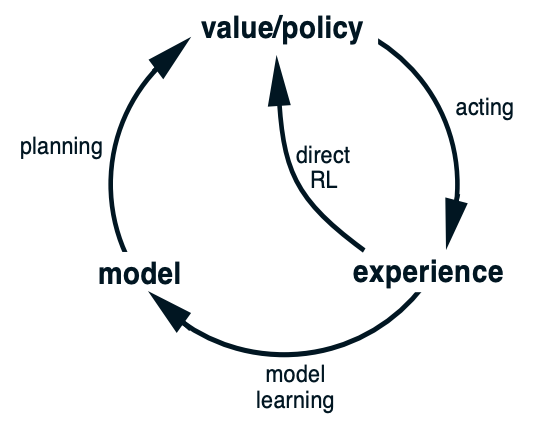
\includegraphics[width=0.5\textwidth]{/chapter8_2}
	\caption{Direct RL and model-learning, either achieved using data collected from experience}
	\label{fig: direct rl and model-learning}
\end{figure}

\begin{figure}
	\centering
	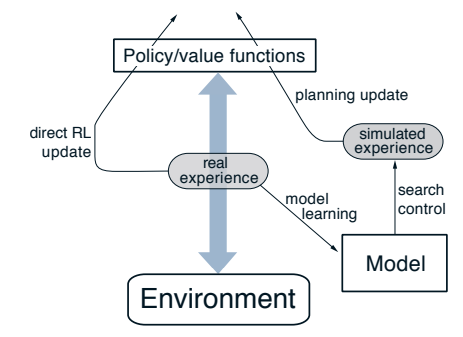
\includegraphics[width=0.75\textwidth]{/chapter8_3}
	\caption{Generalised Dyna architecture}
	\label{fig: dyna}
\end{figure}

\subsection{When the Model is Wrong}
Often our model will be wrong. This can happen initially because the environment is stochastic and we haven't collected enough samples to evaluate this stochasticity accurately. Otherwise, it can happen because we've used function approximation (e.g. neural networks) to predict the model, which generally arrive with non-zero error. When the model is incorrect the planning process is likely to compute a suboptimal policy. Often the suboptimal policy quickly leads to the discovery and correction of modelling error, as when the agent takes actions prescribed by the planned policy in the real environment, it quickly finds the expected rewards are incorrect or do not exist. 

Issues arise when the environment changes to become \textit{better} or more favourable at some stage during learning. In these cases the optimal policy/route to goal remains unchanged, but there is an even better policy available that the agent may never access because it has no reason to doubt its previously learned optimal policy. To address this, another algorithm is proposed called Dyna-Q+. Here, the agent keeps track of the number of timesteps elapsed $\tau$ since a state-action pair had been selected, and, if sufficient time has elapsed, it is presumed that the dynamics of the environment from that state have changed. The modelled rewards for each state-action pair now take the form $r + k\sqrt{\tau}$ for some small $k$.

\subsection{Prioritized Sweeping}
Until now, updates made to the value function during planning have been made arbitrarily, that is to say, state-actions have been sampled uniformly from past experience regardless of how likely we are to visit those state-actions. It would be more useful to prioritize updates to the value function that would be most effected by the reward we have recently received. This general idea is termed \textit{backward focusing} of planning computations. If we prioritize the updates according to a measure of urgency and perform them in order of priority, we call this \textit{prioritized sweeping}. The prioritization queue is assembled based on the expected update to a state-value pair from a new reward. We then loop through this queue, and for each state-value pair, find the state-value pairs we would predict lead to it, and calculated \textit{their} expected update and add them to the queue. The additions to the queue are only made if the expected update is larger than some value $\theta$. In this way, we only plan based on state-value pairs whose value updates are non-trivial. This technique is regularly 5-10 times faster than Dyna-Q.

\subsection{Expected vs. Sample Updates}
This book began by discussing dynamic programming; a way of conducting policy evaluation and improvement given a distribution model of the environment. Then we discussed sampling methods like: Monte Carlo, temporal-difference methods and n-step bootstrapping to estimate value functions in the absence of a model. Implicit here, was the idea that a distribution model than can be used to compute expectations is better than sampling which often leads to higher variance through sampling error. But is this true? To properly assess the relative merits of expected and sample updates for planning we must control for their different computational requirements.

In practice, the computation required by update operations is usually dominated by the number of state-action pairs at which $Q$ is evaluated. For a particular starting pair, $s, a$, let $b$ be the \textit{branching factor} (i.e. the number of possible next states, $s'$ for which $\hat{p}(s|s,a)>0$. Then an expected update of this pair requires roughly $b$ times as much computation as a sample update. If we have sufficient time to complete an expected update, it is usually better than that of $b$ sample updates because of the absence of sampling error. But if there is insufficient time, sampling is always better because some update is better than no update. The key question is therefore: given a unit of computational power, is it better to perform one expected update, or $b$ sample updates? An answer to this question is provide in Figure \ref{fig: samples vs expectations}. For large values of $b$ sampling has huge efficiency gains over expected updates. In reality this effect would be more pronounced as the values of the successor states would be estimates that are themselves updated. By causing estimates to be more accurate sooner, sample updates will have a second advantage in that the values backed up from the successor states will be more accurate.

\begin{figure}
	\centering
	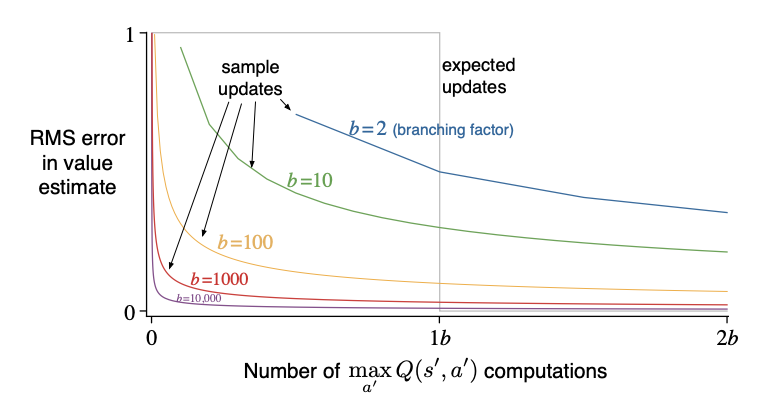
\includegraphics[width=\textwidth]{/chapter8_4}
	\caption{Comparison of efficiency of expected and sample updates}
	\label{fig: samples vs expectations}
\end{figure}

\subsection{Trajectory Sampling}
One could update every state-action pair, or state value, by performing full sweeps of the state space using dynamic programming. As discussed on several occasions this is computationally inefficient, given many of the states may have small probability of occurring. Instead we could sample from state-action space according to some distribution; uniformly in the case of Dyna Q, or according to an on-policy distribution that we observed following the current policy. We can do so by interacting with the model, simulating explicit individual trajectories and updating state or state-action pairs encountered along the way. We call this \textit{trajectory sampling}.

A question arises around whether on-policy updates, that follow the model's transition distribution, are better than updates made with uniform probability across the state-space. It seems for problems with large state-spaces, and small branching factors, it is advantageous to use on-policy distribution sampling. In the long run, however, focusing on the on-policy distribution may hurt because our estimates for these values are already well defined and we are not seeing unusual parts of the state space.

\subsection{Real-time Dynamic Programming}
Real-time dynamic programming (RTDP) is an on-policy trajectory-sampling version of the value iteration algorithm of dynamic programming (DP). Because the algorithm follows the on-policy distribution, our value iteration updates are more efficient that normal DP because we implicitly ignore irrelevant states to our policy in our updates. RTDP is guaranteed to find a policy that is optimal on the relevant states without visiting every state infinitely often, or even without visiting some states at all, under certain conditions. These are:
\begin{itemize}
	\item The initial value of every goal state is zero
	\item There exists at least one policy that guarantees that a goal state will be reached with probability one from any start state.
	\item All rewards for transitions from non-goal states are strictly negative, and
	\item All the initial values are equal to, or greater than, their optimal values (which can be satisfied by setting initial values to 0.)
\end{itemize}

Tasks with these properties are usually called \textit{stochastic optimal path problems}. RTDP can find optimal policies for these tasks with approximately 50\% of the computation required for traditional sweep-based value iteration i.e. dynamic programming.

\subsection{Planning at Decision Time}
The techniques discussed thus far have involved planning in between action-selection, we call this \textit{background planning}. Another way to do planning is at the time of action-selection i.e. to run trajectories or simulations in our model, and decide the optimal action to select based on the outcome of these trajectories. We call this \textit{decision-time planning}.

So we now have two ways of thinking about planning:
\begin{enumerate}
	\item Using simulated experience to gradually improve our policy or value function, or
	\item Using simulated experience to select an action for the current state
\end{enumerate}

Usually the results of this kind of planning are not used to update our value function or policy directly, and are generally discarded after action selection. This is fine for large state spaces, but if the state spaces are smaller than it can be expedient to keep these values and update our value function, such that we combine the two types of planning outlined above.

Decision-time planning is most useful in applications where fast response is not required, like chess. If low-latency actions are required, it's generally better to do planning in the background.

\subsection{Heuristic Search}
The canonical decision time planning method is \textit{heuristic search}. For each state encountered, heuristic search dedicates computational resource to searching a large tree of possible continuations, or state permutations thereafter. The search evaluates leaf nodes at the end of the search and backs up the values to the state-action nodes for the current states. The value maximising action from the current state is found and then selected. The values are usually discarded. This kind of planning is effective because it focuses only on pertinent next states and actions, and focuses resource on obtaining the next best one-step action. The backup diagram for heuristic search is shown in Figure \ref{fig: heuristic search}.

\begin{figure}
	\centering
	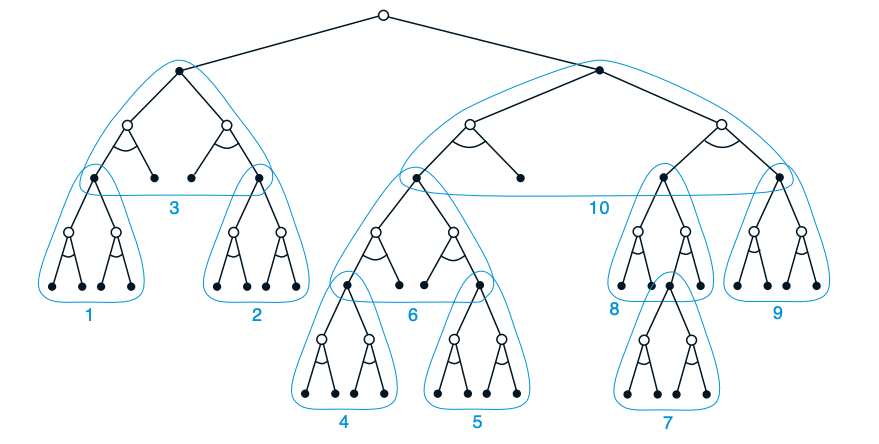
\includegraphics[width=\textwidth]{/chapter8_5}
	\caption{Heuristic search can be implemented as a sequence of one-step updates (shown here outlined in blue) backing up values from the leaf nodes toward the root. The ordering shown here is for a selective depth-first search.}
	\label{fig: heuristic search}
\end{figure}

\subsection{Rollout Algorithms}
Rollout algorithms apply Monte Carlo control to simulated trajectories that all begin at the current environment state. They estimate action values for a given policy by averaging the returns from many simulations in a model using the current policy. These algorithms, like heuristic search, make immediate use of these action value estimates then discard them, they do not attempt to estimate $q_*$ like Monte Carlo policy iteration as discussed in chapter 5. They take advantage of the mathematical properties of policy iteration discussed in chapter 4, that is, $\pi'$ > $\pi$ if both are identical except that $\pi'(s) = a \neq \pi(s)$ and $q_{\pi}(s,a) \geq v_\pi(s)$.

The limited factor with these types of algorithms is always computational resource, which itself is dependent on the size of the state-space. However there are ways around this, including pruning the rollouts to only involve the most probable next states, or to truncate simulated trajectories so they do not run to the end of the episode.

\subsection{Monte Carlo Tree Search}
Monte Carlo Tree Search (MCTS) is a rollout algorithm as described above, but with some modifications. Instead of rolling out trajectories randomly, MCTS first selects a small set of actions according to its \textit{tree policy}, then sometimes expands this selection to one or more actions, and then performs a full rollout to end of episode using a rollout policy. The value found upon termination of this trajectory is then backed up to the current state. This process is repeated for as long as time/computational constraints allow, then the agent selects an action usually based on which action produced best future estimated reward. MCTS is illustrated in Figure \ref{fig: MCTS}

\begin{figure}
	\centering
	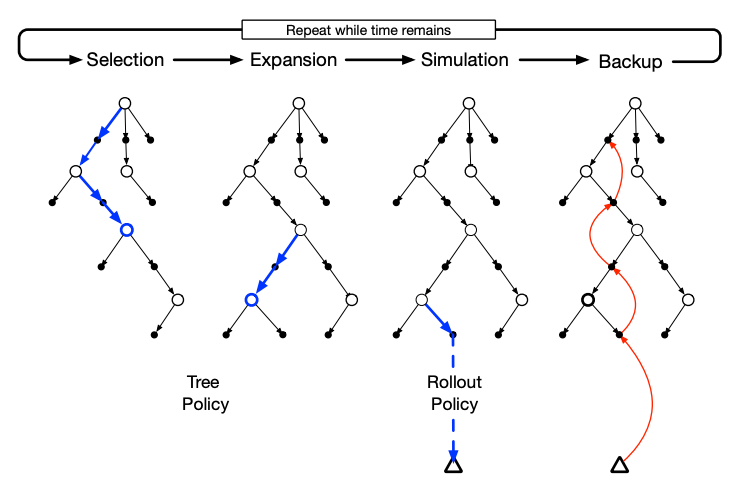
\includegraphics[width=\textwidth]{/chapter8_6}
	\caption{Monte Carlo Tree Search. When the environment changes to a new state, MCTS executes as many iterations as possible before an action needs to be selected, incrementally building a tree whose root node represents the current state. Each iteration consists of the four operations Selection, Expansion (though possibly skipped on some iterations), Simulation, and Backup, as explained in the text and illustrated by the bold arrows in the trees.}
	\label{fig: MCTS}
\end{figure}

\subsection{Key Takeaways}
\begin{itemize}
	\item Planning algorithms use models. These models can be either \textit{distribution models} that provide a probability distribution over next states (as required to compute expectations for dynamic programming), or can be \textit{sample models} that provide a sample of future states drawn from the underlying distribution that we are yet to access, or cannot access.
	\item Algorithms used for both learning and planning are often identical, the difference being that \textit{learning} involves updating our value function from real experience, whereas \textit{planning} involves updating our value function based on simulated experience from our model.
	\item Models can often be wrong, and the best way to ensure they stay up to date in continual maintain them through true experience. Sometimes we will obtain an optimal policy using a model that was once correct, but has since become redundant. We can attempt to keep an accurate model of our environment by taking actions in the environment that have not be attempted for some time to test the truth of our model. This technique is exhibited by Dyna Q+.
	\item Sample updates are often more efficient than expected updates for large state-spaces with large branching factors (a measure of the expected number of possible next states from an action).
	\item Trajectory sampling in our model can be used for planning. This can be useful when conducted on-policy, because we prioritise making updates to our value function that are particularly relevant to our policy.
	\item Planning can be conducted pre-action selection, to update our value function and inform future action-selection, or it can be done at the time of action-selection. The former is called \textit{background planning} and the latter is called \textit{decision time planning}.
	\item Examples of decision time planning include Heuristic Search (where value maximising actions are taken in a simulation of various next states, and backed up to the root node), Rollout Algorithms (where Monte Carlo rollouts are performed over many simulations of episodes and the value maximising action returned), or MCTS (a special case of rollout algorithms that effectively combines heuristic search over some small number of actions and then performs Monte Carlo rollouts thereafter).
	\item Decision time planning can be effective for tasks where low-latency action selection is not required. They are fundamentally limited by the time constraints on action-selection and on the available computational resource.
\end{itemize}

\subsection{Summary of Part I}
Each of the methods presented this far in this textbook can be summarised on the continuum illustrated in Figure \ref{fig: part1 summary}.

\begin{figure}
	\centering
	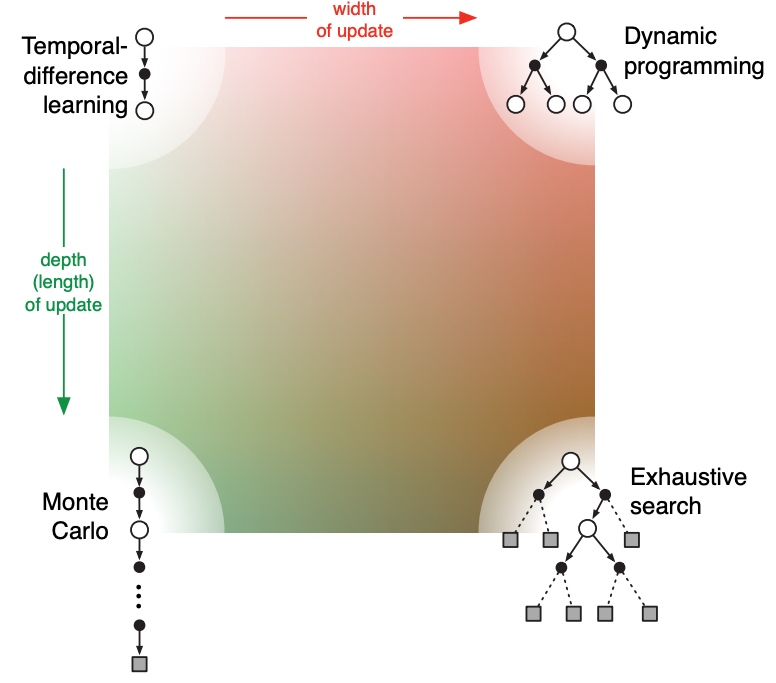
\includegraphics[width=0.75\textwidth]{/chapter8_7}
	\caption{A slice through the space of reinforcement learning methods, highlighting the two of the most important dimensions explored in Part I of this book: the depth and width of the updates.}
	\label{fig: part1 summary}
\end{figure}

